\subsection{有限次扩张的可分次数与不可分次数}

设 E 是 K 的有限次扩张，\(\Omega\) 是 K 的一个代数闭包。回顾（V，第 31 页），所谓 E 在 K 上的可分次数，记作 \([E:K]_{s}\) ，是指 E 到 \(\Omega\) 中的 K-同态的个数。

命题 15.——设 \(\mathbf{E}_s\) 是 \(\mathbf{K}\) 在 \(\mathbf{E}\) 中的相对可分闭包；则 \([\mathbf{E}:\mathbf{K}]_s = [\mathbf{E}_s:\mathbf{K}]\) .

域 \(\Omega\) 是完全的，且 \(E\) 是 \(p\) -根式的（在 \(E_s\) 上），这依据 \(V\) 第 44 页命题 13；因此命题 3（V，第 26 页）表明，\(E_s\) 到 \(\Omega\) 中的每个 K-同态都能以唯一方式延拓为 \(E\) 到 \(\Omega\) 中的 K-同态；于是我们有 \([E:K]_s = [E_s:K]_s\) 。由于 \(E_s\) 是 \(K\) 的有限次可分扩张，它是 \(K\) 上的平展代数；故 \([E_s:K]_s = [E_s:K]\) （由 \(V\) ，第 32 页，命题 4），结论得证。

沿用前面的记号，E 在 \(E_{s}\) 上的次数称为 E 在 K 上的不可分次数，记作 \([E:K]_{i}\) 。于是我们有

\[
[ \mathrm{E}: \mathrm{K} ] = [ \mathrm{E}: \mathrm{K} ] _ {s} \cdot [ \mathrm{E}: \mathrm{K} ] _ {i}\tag{1}
\]

由命题 15。

\pandocbounded{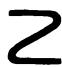
\includegraphics[keepaspectratio]{images/part001_fb7ec604.jpg}}

当 K 的特征为 0 时，有 \(E = E_{s}\) ，因此 \([E : K]_{s} = [E : K]\) 且 \([E : K]_{i} = 1\) 。若 K 的特征为 \(p \neq 0\) ，则数 \([E : K]_{i}\) 是 p 的幂，因为 E 在 \(E_{s}\) 上是 p-根式扩张（V，第 44 页，命题 13 及第 26 页，命题 4）。应当注意，\([E : K]_{i}\) 未必等于整除 \([E : K]\) 的 p 的最高次幂，也未必等于 E 在 K 中的相对 p-根式闭包的次数 \([E_{r} : K]\) （V，第 152 页，习题 3 和 2）。

命题 16.——设 \(\Omega\) 是 K 的一个扩张，E、F 是 \(\Omega\) 的两个子扩张，在 K 上次数有限。

\begin{enumerate}
\def\labelenumi{\alph{enumi})}
\item
  若 \(\mathrm{E} \subset \mathrm{F}\) ，则 \([\mathrm{F}:\mathrm{K}]_s = [\mathrm{F}:\mathrm{E}]_s \cdot [\mathrm{E}:\mathrm{K}]_s\) 且 \([\mathrm{F}:\mathrm{K}]_i = [\mathrm{F}:\mathrm{E}]_i \cdot [\mathrm{E}:\mathrm{K}]_i\) .
\item
  设 \(\mathbf{K}'\) 是 \(\Omega\) 的一个子扩张；则我们有
\end{enumerate}

\[
\left[ \mathrm{K} ^ {\prime} (\mathrm{E}): \mathrm{K} ^ {\prime} \right] _ {s} \leqslant \left[ \mathrm{E}: \mathrm{K} \right] _ {s} \quad \text{且} \quad \left[ \mathrm{K} ^ {\prime} (\mathrm{E}): \mathrm{K} ^ {\prime} \right] _ {i} \leqslant \left[ \mathrm{E}: \mathrm{K} \right] _ {i},
\]

且当 \(\mathbf{K}'\) 与 \(\mathbf{E}\) 在 \(\mathbf{K}\) 上线性不相交时等号成立。

\begin{enumerate}
\def\labelenumi{\alph{enumi})}
\setcounter{enumi}{2}
\tightlist
\item
  我们有 \([\mathrm{K}(\mathrm{E}\cup \mathrm{F}):\mathrm{K}]_s\leqslant [\mathrm{E}:\mathrm{K}]_s.\) \([\mathrm{F}:\mathrm{K}]_s\) 且 \([\mathrm{K}(\mathrm{E}\cup \mathrm{F}):\mathrm{K}]_i\leqslant [\mathrm{E}:\mathrm{K}]_i.\) \([\mathrm{F}:\mathrm{K}]_i\) ，且当 E 与 F 在 K 上线性不相交时等号成立。
\end{enumerate}

\(a\) 中关于可分次数的断言由 (9)（V，第 32 页）可得。由于 \([F:K] = [F:E].[E:K]\) ，关于不可分次数的断言由此及 (1) 得出。

由命题 13 的推论 1（V，第 44 页）及命题 15，我们有

\[
\left[ \mathrm{K} ^ {\prime} (\mathrm{E}): \mathrm{K} ^ {\prime} \right] _ {s} = \left[ \mathrm{K} ^ {\prime} \left(\mathrm{E} _ {s}\right): \mathrm{K} ^ {\prime} \right], \quad \left[ \mathrm{K} ^ {\prime} (\mathrm{E}): \mathrm{K} ^ {\prime} \right] _ {i} = \left[ \mathrm{F} ^ {\prime} (\mathrm{E}): \mathrm{K} ^ {\prime} \left(\mathrm{E} _ {s}\right) \right];\tag{2}
\]

当 \(K'\) 在 K 上与 E 线性不相交时，\(E_{s}\) 在 K 上与 \(K'\) 线性不相交，且 E 与 \(\mathrm{K}'(\mathrm{E}_{s})\) 在 \(E_{s}\) 上线性不相交（V，第 15 页，命题 8）。断言 b) 现由命题 5（V，第 14 页）得出。

由 a) 我们有 \([\mathbf{K}(\mathbf{E}\cup\mathbf{F}):\mathbf{K}]_{s}=[\mathbf{F}(\mathbf{E}):\mathbf{F}]_{s}\cdot[\mathbf{F}:\mathbf{K}]_{s}\) ；由 b) 我们有 \([\mathbf{F}(\mathbf{E}):\mathbf{F}]_{s}\leqslant[\mathbf{E}:\mathbf{K}]_{s}\) ，且当 E 与 F 在 K 上线性不相交时取等号。因此我们得到不等式 \([\mathbf{K}(\mathbf{E}\cup\mathbf{F}):\mathbf{K}]_{s}\leqslant[\mathbf{E}:\mathbf{K}]_{s}\cdot[\mathbf{F}:\mathbf{K}]_{s}\) ，且当 E 与 F 在 K 上线性不相交时取等号。c) 中关于不可分次数的断言可用类似的方式证明。

